\documentclass[12pt]{exam}
\usepackage{epsfig}
\usepackage[usenames,dvipsnames,svgnames,table]{xcolor}
\usepackage{listings}
\usepackage{color}
\usepackage{float}
\usepackage{subfig}

\usepackage[bookmarksopen=true]{hyperref}

\newcommand{\note}[1]{\marginpar{\LARGE $\spadesuit$}
      $\spadesuit$ {\bf #1} $\spadesuit$}
      
\lstdefinestyle{error}{
  emptylines=1,
  breaklines=true,
  basicstyle=\ttfamily\color{red}
}

\lstdefinestyle{command}{
  emptylines=1,
  breaklines=true,
  basicstyle=\ttfamily\color{black}
}

% Please use ctrl or cmd F to find all inshttps://www.overleaf.com/project/604b1e9e44ce1d73e3aed4ddtances of the pound symbol #, and replace with the appropriate assignment number. Similarly for 'DATE' for the assignment due date. 

% To compile and produce a PDF from tex files please look to homebrew and install the appropriate latex libraries. 

\pagestyle{headandfoot}
\firstpageheader{}{}{}
\runningheader{CPSC 314}{Assignment 4}{Due 11:59pm on March 28th, 2022}
\footer{}{Page \thepage\ of \numpages}{}
\setlength{\parindent}{0pt}
\begin{document}

% Give your assignment a title. 

\title{CPSC 314\\
  Assignment 4: Textures and Shadows}
\date{Due 11:59PM, March 28th, 2022}

\maketitle

\section{Introduction}

% What are students expected to do?
% What are students expected to learn?
% Optionally include a graphic to explain the scene if it helps.

In this assignment you will be learning about different uses of textures. You will implement a skybox, as well as give your favourite armadillo a new, dazzling look, and make it cast shadows. And you'll meet a new protagonist, Shay D. Pixel, a SIGGRAPH mascot, and get a taste of physically based rendering and image-based lighting.

\subsection{Getting the Code}

Assignment code is hosted on the UBC Students GitHub. To retrieve it
onto your local machine navigate to the folder on your machine where you intend to keep your
assignment code, and run the following command from the terminal or command line:

\medskip
{\tt git clone https://github.students.cs.ubc.ca/cpsc314-2021w-t2/a4-release.git}

\subsection{Template}

\begin{itemize}

\item The file {\tt A4.html} is the launcher of the assignment. Open it in your preferred browser to run the assignment, to get started.

\item The file {\tt A4.js} contains the JavaScript code used to set up the scene and the rendering
    environment.

\item The folder {\tt glsl} contains the vertex and fragment shaders.

\item The folder {\tt js} contains the required JavaScript libraries. You do not need to change anything here.

\item The folder {\tt gltf} contains the geometric models loaded in the scene.

\item The folder {\tt images} contains the texture images used.

\end{itemize}

\section{Work to be done (100 points)}

First, ensure that you can run the template code in your browser. See
instructions in Assignment 1. The initial scene should look as in Figure~\ref{fig:init}.\\

\begin{figure}[ht]
  \centering
  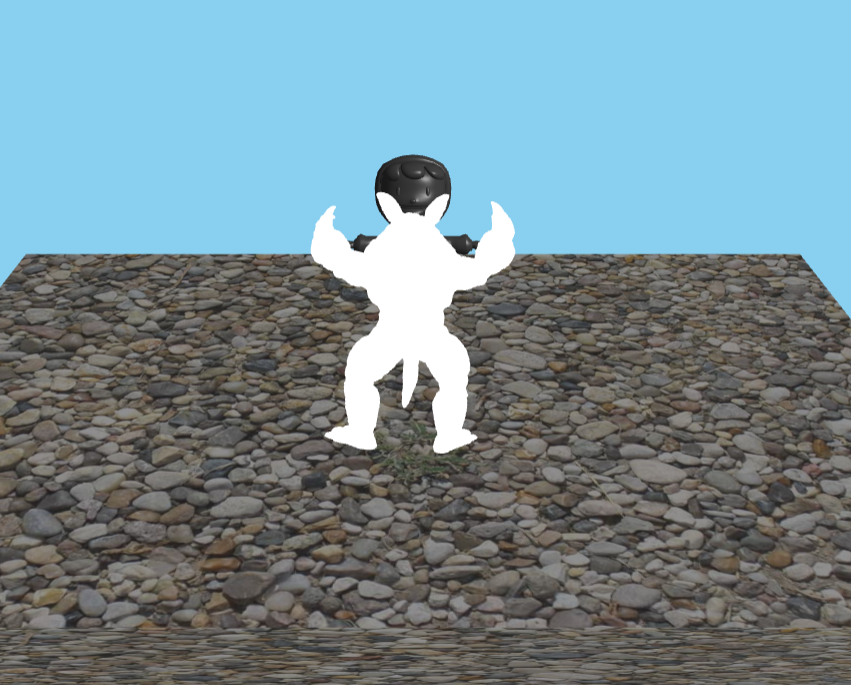
\includegraphics[width=0.5\textwidth]{./init.png}
    \caption{Initial configuration\label{fig:init}}
\end{figure}

\begin{enumerate}

\item {\bf Part 1: Required Features}

  \begin{enumerate}

\item {\bf (15 points)} Texture Mapping with ShaderMaterial.

In this part you will implement texture mapping for Shay D. Pixel using shaders. You are provided with a color texture \texttt{images/Pixel\_Model\_BaseColor.jpg}. The geometric model has vertex UV coordinates baked in. The model is read from a \texttt{glTF} file, a new format that is growing in popularity. We have provided the loader so you don't have to know details of how glTF works.
  
Your task is to:
\begin{itemize}
    \item Pass the textures (as a uniform) to the \texttt{shay.fs.glsl} fragment shader and use the right UV coordinates to sample a color from the texture. Use this sampled color and the light intensity (which is computed for you in \texttt{shay.fs.glsl}) to calculate the final fragment color.
\end{itemize}

\textit{Hint 1:} Here, the texture is flipped on the y-axis. Take this into consideration when you assign the UV coordinates.
\begin{figure}[H]
  \centering
  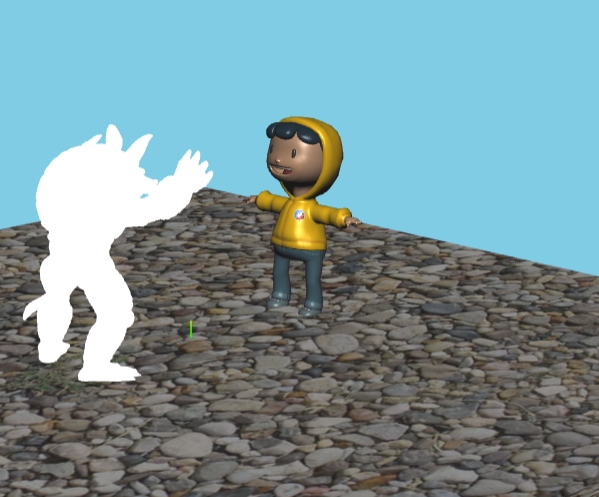
\includegraphics[width=0.5\textwidth]{./part-aii.png}
  \caption{Question 1a) Texture mapping with ShaderMaterial\label{fig:part-aii}}
\end{figure}

    
\item {\bf (15 points)} Skybox.

A skybox is a simple way of creating backgrounds for your scene with textures. We have provided six textures in \texttt{ images/pos[x/y/x].png \& images/neg[x/y/z].png}. You will implement a skybox using cube environment mapping as discussed in class, where you map these textures on to a large cube surrounding the scene. You need to load the six textures to \texttt{skyboxCubemap} in the proper order, you can pass this as a \texttt{samplerCube} uniform to complete the \texttt{skybox} shaders. Sampling is done using the overloaded \texttt{texture()} function. To sample a \texttt{samplerCube} object, you require a texture and a direction. 
 In this case the texture coordinate input is replaced by the viewing direction for the specific fragment.

For this question, you will be completing the \texttt{skybox.vs.glsl} and \texttt{skybox.fs.glsl}. Note that while the material and shaders are already loaded, it's your task to create the correct geometry and add it to the scene as you did in the previous assignments. 

\textit{Hint 1:} The skybox should move with the camera, so that it always is in front of the camera. \\
\textit{Hint 2:} Cubemaps are sampled using a direction vector. Think about which vector you can use for this.

\begin{figure}[H]
  \centering
  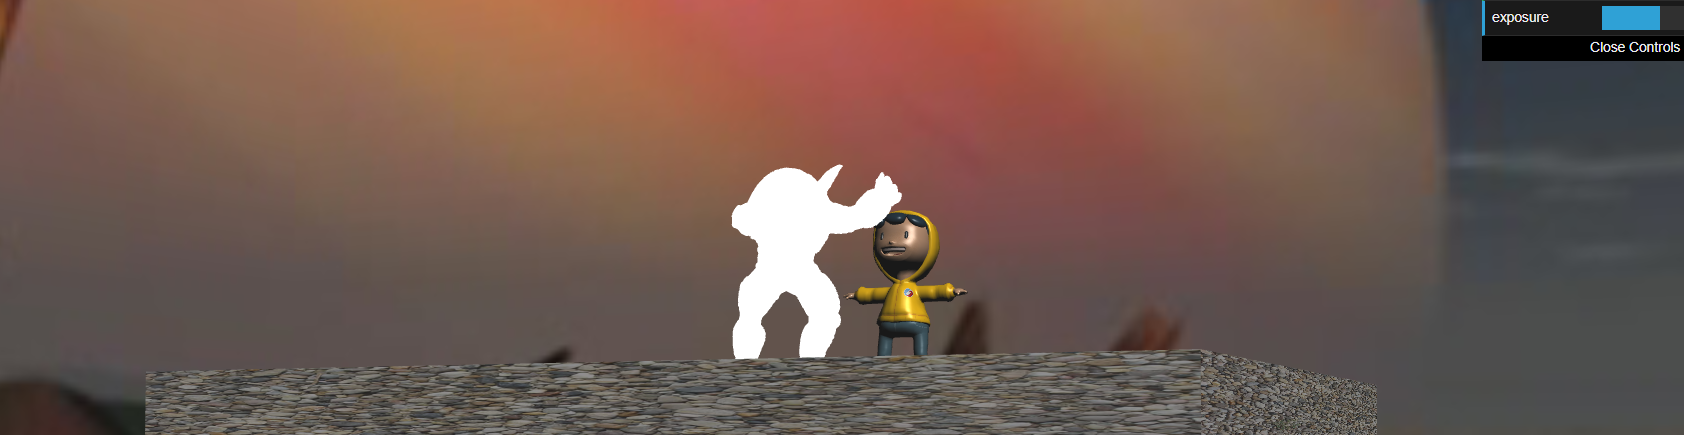
\includegraphics[width=0.5\textwidth]{./part-b.png}
  \caption{Question 1b). Skybox.\label{fig:skybox}}
\end{figure}




\item {\bf (20 points)} Shiny Armadillo.

Another interesting use of \texttt{samplerCubes} is \textbf{environment mapping}. This can be used to make the same, boring armadillo highly reflective, like a mirror. For this part, complete the shaders \texttt{envmap.vs.glsl} and \texttt{envmap.fs.glsl} to implement a basic reflective environment map shader.

You can use the same cube texture \texttt{skyboxCubemap} in your shaders which is passed as a \texttt{samplerCube} uniform like before, as well as the same \texttt{texture()} function, but pay attention to use the correct \texttt{vec3}, described in class and in the textbook, to retrieve the texture color. 

\textit{Hint 1:} Try replacing the armadillo with a sphere object to start off with so it is easier to inspect and debug your environment map. \\
\textit{Hint 2:} Think about how the armadillo (or sphere) should look from various directions. How should it look from the bottom? The top?


\begin{figure}[H]
  \centering
  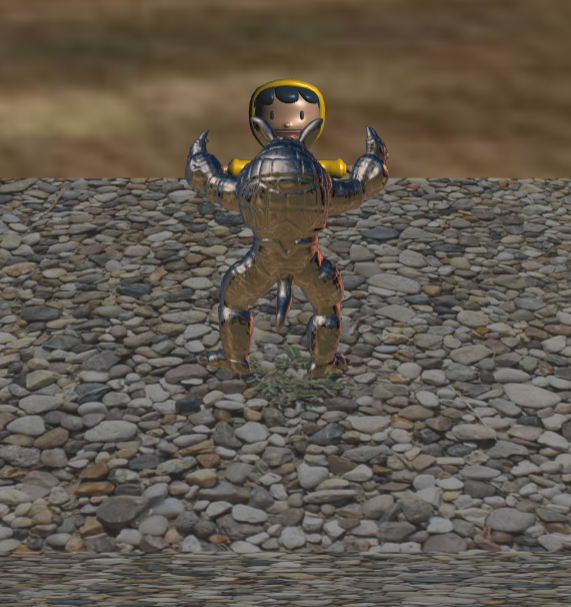
\includegraphics[width=0.42\textwidth]{./part-c.png}
  \caption{Question 1c). Shiny Armadillo.\label{fig:part-c}}
\end{figure}

\item {\bf (35 points)} Shadow Mapping.

Shadows are a tricky part of computer graphics, since it is not easy to figure out
which parts of a scene should be cast in shadow. There are many techniques to
create shadows (raytracing, shadow volumes, etc.). In this assignment, we will use
shadow mapping. Shadow mapping is all about exploiting the z-buffer. A shadow
map is rendered in an off-screen frame buffer by projecting the scene from the
perspective of a light source, giving us a depth-like value at each fragment along
rays of the light source.
For this section of the assignment, you will do a hands-on implementation of
shadow mapping. Your goal will be to get the armadillo and ShayD to cast smooth
shadows onto the floor. You can switch between scene views by pressing keys 1, 2, and
3 for the scene, depth scene, and shadowed scene respectively (scenes 2 and 3 are for
you to implement).

\begin{enumerate}
\item Start by creating the shadow map, which is the depth map when viewed from the camera. Add the appropriate objects to the provided shadowScene, do a first pass render to a WebGLRenderTarget to create the depth map, and finally visualise this using the provided postScene (short for ``post processing scene''). Your primary job will be to pass the appropriate textures between render targets and to implement the render.vs/fs shaders. You will find the API docs useful.
\newline
\url{https://threejs.org/docs/#api/en/renderers/WebGLRenderTarget}
    \item Next, use the depth map to project the shadows onto the floor. This will involve modifying the floor shader code to check whether a fragment is in shadow or outside. You can do this by transforming the fragment's position to ``light space'' (i.e., in the shadow camera's coordinate frame), and using that to compute the appropriate texture coordinate in the shadow map. Then compare the depth of the fragment to the value stored in the shadow map.
    \item Lastly, you will smooth the shadows by using percentage closer filtering (PCF), in
the floor shader code. PCF is a shadow anti-aliasing technique which reduces `jaggies'
by replacing the binary in/not-in shadow calculation of a pixel, with a calculation that
instead checks if a pixel and its neighbours are in shadow, and `shadows' the pixel
according to the fraction that are.

\end{enumerate}

\begin{figure}[H]
  \centering
  
\includegraphics[width=0.5\textwidth]{./part-d.png}
    \caption{Question 1d) (i). Depth Map.\label{fig:part-d}}
\end{figure}

\begin{figure}[H]
  \centering
  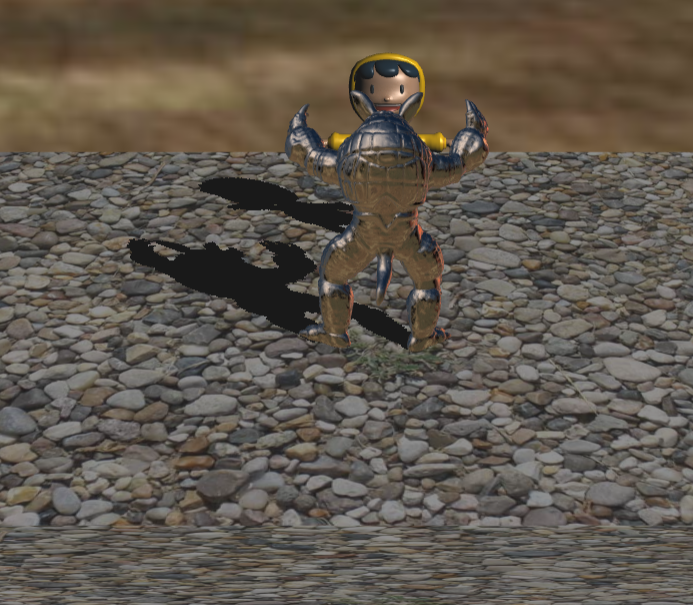
\includegraphics[width=0.5\textwidth]{./part-e.png}
    \caption{Question 1d) (ii). Shadow mapping.\label{fig:part-e}}
\end{figure}

\begin{figure}[H]
  \centering
  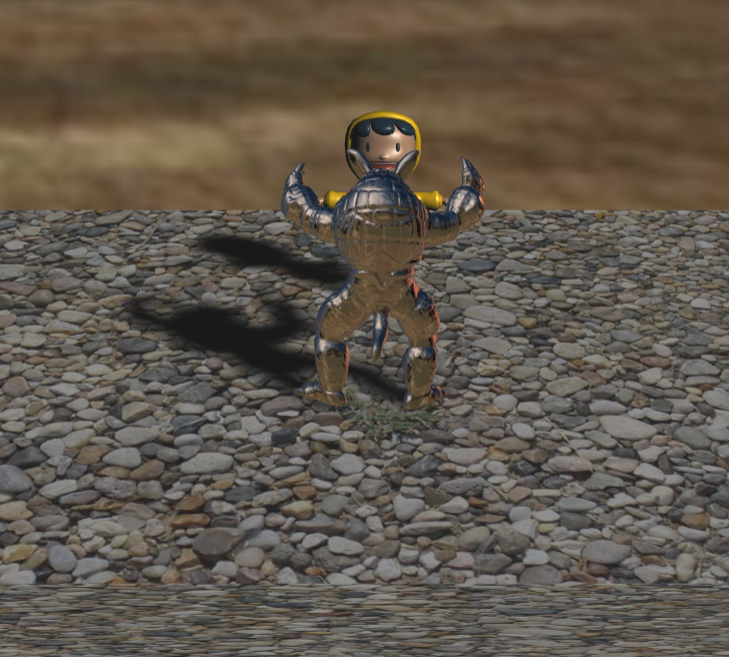
\includegraphics[width=0.5\textwidth]{./part-f.png}
    \caption{Question 1d) (iii). Shadow mapping smooth.\label{fig:part-eiii}}
\end{figure}

\end{enumerate}

\item {\bf (15 points)} Image-based Lighting

Image-based lighting (IBL) is a rendering technique which requires capturing real-world light information as a High Dynamic Range (HDR) image. This image is then used to calculate the lighting for objects in the scene. IBL can create incredibly realistic simulations of real world lighting, especially when used with physically based materials as we discussed in class. You will set up a scene in three.js to use IBL. You can enter the IBL scene by pressing the key 4. 

\begin{figure}[H]
  \centering
  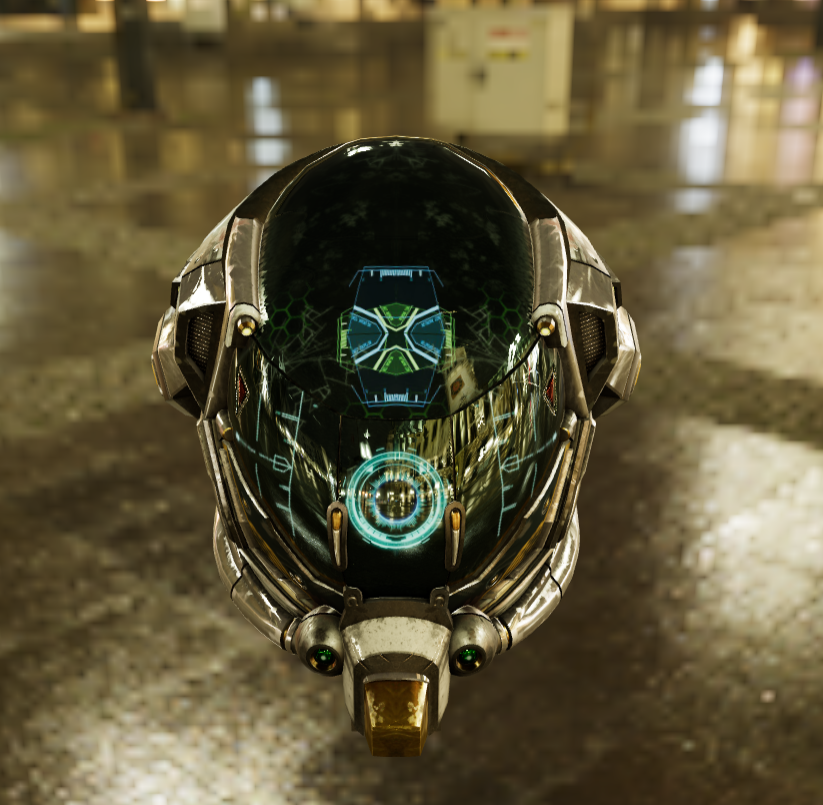
\includegraphics[width=0.5\textwidth]{./part-a.png}
  \caption{Complete IBL scene\label{fig:part-a}}
\end{figure}

 Even though this can be complicated we have made the problem as simple as possible so that you can get a flavor for how to use these techniques, without getting bogged down. Your tasks are:
\begin{itemize}
    \item Set up \texttt{helmetMaterial} by loading the individual textures of the helmet and setting the corresponding properties of the material.
    \item Complete \texttt{helmetMaterial} by setting the material's environment map property after loading the HDR texture.
\end{itemize}


\newpage

\item {\bf (10 points max)} Part 2: Creative License (Optional)

You have many opportunities to unleash your creativity in
computer graphics!  In this \textbf{optional} section, and you are
invited to extend the assignment in fun and creative ways.
We'll highlight some of the best work in class. A number of
exceptional contributions may be awarded bonus points.
Some possible suggestions might be:
\begin{itemize}
  % give students suggestions for creative components, look at previous assignments for ideas. 
\item Experiment with multi-pass rendering to create a texture out of the current scene to use for the armadillo environment map, such that the armadillo appears to reflect the objects in its surroundings.
\item Experiment with other graphics techniques, like procedural mapping (eg. Perlin noise), subsurface scattering (``Gaussian blur"), ambient occlusion, and raytracing.
\item Make a short film/animation and tell a tear-jerking story with sounds.
\item Make an interactive video game.
\end{itemize}

\end{enumerate}

\section{Submission Instructions}
\subsection{Directory Structure}
Under the root directory of your assignment, create two subdirectories
named ``part1'' and ``part2'', and put all the source files, your
makefile, and everything else required to run each part in the respective
folder. Do not create more sub-directories than the ones already provided. 

You must also write a clear README.txt file that includes your name,
student number, and CWL username, instructions on how to use the
program (keyboard actions, etc.) and any information you would like to
pass on to the marker. Place README.txt under the root directory of your
assigment.

\subsection{Submission Methods}
Please compress everything under the root directory of your assignment into
{\tt a4.zip} and submit it on Canvas. You can make multiple submissions,
but we will grade only the last one.

\section{Grading}
\subsection{Point Allocation}
Each assignment has 100 points for Part 1. Part 2 is optional and you can get bonus points (0-10 points) if the work is noteworthy; there are no points for ``effort''.
Percentage wise, we use Part 1's total points as the denominator: e.g. if you
get 95 out of 100 points from Part 1, but no points from Part 2, then your percentage
grade would be 95/100. If you get full points from both Parts, then your percentage
grade would be 110/100.

\subsection{Face-to-face (F2F) Grading}
For each assignment, you are required to meet face-to-face with a TA in person or on Zoom
to demonstrate that you understand why your program works. Details regarding how to
sign up a grading session with a TA will be annouced on Canvas and Piazza.

\subsection{Penalties}
Aside from penalties from incorrect solution or plagiarism, we may apply the following
penalties to each assignment:

\textbf{Late penalty.} You are entitled to three grace (calendar) days in total
throughout the term. No penalties would be applied for using them. However once
you have used up the grace days, a deduction of 10 points would be applied to each
extra late day. Note that
\begin{enumerate}
  \item The three grace days are given for all assignments, \textbf{not per assignment}, so please use them wisely;
  \item We consider the time of only your last submission;
  \item We do not consider Part 1 and Part 2 submissions separately. Say if you submitted Part 1 on time but updated your submission for Part 2 one day after the deadline, we would count one late day.
\end{enumerate}

\textbf{No-show penalty.} You are required to sign up a grading slot at least one day
before F2F grading starts, and show up at your slot on time. So a 10-point deduction would
be applied to each of the following circumstances:
\begin{enumerate}
  \item Not signing up a grading slot before the sign-up period closes;
  \item Not showing up at your grading slot.
\end{enumerate}
Note that we would not apply the penalty if you are unable to sign up/show up on time
due to an emergency, or if you cannot sign up because none of the slots work for you.
In those cases, please contact the course staff immediately on Piazza.

\end{document}
%%% Local Variables:
%%% mode: latex
%%% TeX-master: t
%%% End:
